\documentclass[twocolumn]{scrartcl}
%\documentclass{scrartcl}

\usepackage[utf8]{inputenc}
\usepackage[T1]{fontenc}
\usepackage{lmodern}
\usepackage[ngerman]{babel}
\usepackage{amsmath}

\usepackage{makeidx}
\makeindex

\usepackage{fancyvrb}
\usepackage{fvextra}

\usepackage[sc]{mathpazo} % or option osf
\usepackage{newpxmath}
\usepackage[output-decimal-marker={,}]{siunitx}

\usepackage[comma,authoryear]{natbib}
\bibliographystyle{natdin}

\usepackage{adjustbox}
\usepackage[a4paper, margin=1mm, includefoot, footskip=15pt]{geometry}
\usepackage{afterpage}

\usepackage{pgfplotstable}
\usepackage{tikz}
\usepackage{array}
\usepackage{arydshln}

\usepackage[pdftitle={Kriterien und Hilfen bei der Baumartenwahl}
, pdfauthor={Georg Kindermann}
, pdfsubject={Waldbau, Waldwachstum}
, pdfkeywords={Waldbau, Waldwachstum, Wald, Forst}
, pdflang={de-AT-1996}
, hidelinks
, pdfpagemode=None]{hyperref}

\nonfrenchspacing
\sloppy
\usepackage{breqn}
\usepackage{enumitem}
%\usepackage{rotating}
\usepackage{pdflscape}

\usepackage{pdfpages}

\title{Kriterien und Hilfen bei der Baumartenwahl}
\author{Georg Kindermann}

\newlength{\eX}
\settoheight{\eX}{X}
\newcommand*{\torte}[1]{\begin{tikzpicture}[baseline={([yshift=2pt]current bounding box.south)},line width=1pt]%
    \ifnum0=#1 \else
    \ifnum1=#1 \draw (0,0) circle (.5\eX); \else
    \draw (0,0) circle (.5\eX);
    \fill (0,0) -- (90:.5\eX) arc (90:90-(#1-1)*72:.5\eX) -- cycle;
    \fi\fi
  \end{tikzpicture}}

\newcommand*{\hst}[1]{\begin{tikzpicture}[baseline={([yshift=2pt]current bounding box.south)},line width=1pt]
    %\path (0,0) (1em,1.0em);
    \ifnum4=#1\draw (.5\eX,1\eX) -- (0\eX,0\eX) -- (1\eX,0\eX) -- cycle;\else
    \ifnum3=#1\draw[fill] (.3\eX,1\eX) -- (.15\eX,.5\eX) -- (.85\eX,.5\eX) -- (.7\eX,1\eX) -- cycle;
    \draw (.15\eX,.5\eX) -- (0\eX,0\eX) -- (1\eX,0\eX) -- (.85\eX,.5\eX) -- cycle;
    \else
    \ifnum2=#1\draw (.3\eX,1\eX) -- (.15\eX,.5\eX) -- (.85\eX,.5\eX) -- (.7\eX,1\eX) -- cycle;
    \draw[fill] (.15\eX,.5\eX) -- (0\eX,0\eX) -- (1\eX,0\eX) -- (.85\eX,.5\eX) -- cycle;
    \else
    \ifnum1=#1\draw (0\eX,.2\eX) -- (1\eX,.2\eX) {[rounded corners=2pt] -- (1\eX,1\eX) -- (.5\eX,.5\eX)} -- (0\eX,.5\eX) -- cycle;
    \else
    \ifnum0=#1\draw[fill] (0,0) -- (1\eX,0) -- (1\eX,.5\eX) {[rounded corners=2pt] -- (.5\eX,.2\eX)} -- (0,.5\eX) -- cycle;
    \fi\fi\fi\fi\fi
  \end{tikzpicture}
}

\newcommand*{\rating}[1]{\begin{tikzpicture}[baseline={([yshift=2pt]current bounding box.south)},line width=1pt]
    \ifnum0=#1\tikz \draw[rounded corners=2pt] (0,0) rectangle (1em,1em);\else
    \ifnum1=#1\begin{tikzpicture}
      \draw[rounded corners=2pt] (0,0) rectangle (1em,1em);
      \fill[black, radius=.1em] (.5em,.5em) circle;
    \end{tikzpicture} \else
    \ifnum2=#1\begin{tikzpicture}
      \draw[rounded corners=2pt] (0,0) rectangle (1em,1em);
      \fill[black, rounded corners=2pt] (.2em,.2em) rectangle (.8em,.8em);
    \end{tikzpicture} \else
    \ifnum3=#1\tikz \fill[black,rounded corners=2pt] (0,0) rectangle (1em,1em);
    \fi\fi\fi\fi
  \end{tikzpicture}
}

\newcommand{\ratingB}[2]{\begin{tikzpicture}[baseline={([yshift=2pt]current bounding box.south)},line width=1pt,x=1em,y=1em]
    \begin{scope}
      \clip[rounded corners=2pt] (0,0) rectangle (1,1);
      \fill[black] (0,0) rectangle (1,#1/#2);
    \end{scope}
    \draw[rounded corners=2pt] (0,0) rectangle (1,1);
  \end{tikzpicture}%
}

%\usepackage{tabularray} %Maybe in future
\usepackage{xtab}
\newcommand{\ratingC}[2]{\begin{tikzpicture}[baseline={([yshift=2pt]current bounding box.south)},line width=1pt,x=1em,y=1em]
    \begin{scope}
      \clip[rounded corners=2pt] (-.5,-.5) rectangle (.5,.5);
      \draw[fill] (0,0) -- (90-#1/100*360:1) arc (90-#1/100*360:90-#2/100*360:1) -- cycle;
    \end{scope}
    \draw[rounded corners=2pt] (-.5,-.5) rectangle (.5,.5);
  \end{tikzpicture}%
}

\newcommand*{\jaNein}[1]{\begin{tikzpicture}[baseline={([yshift=2pt]current bounding box.south)},line width=1pt,x=1em,y=1em]%
    \ifnum0=#1 \draw[rounded corners=2pt] (-.5,-.5) rectangle (.5,.5); \else
    \ifnum1=#1 \draw[fill,rounded corners=2pt] (-.5,-.5) rectangle (.5,.5);
    \fi\fi
  \end{tikzpicture}}

\newcommand{\jaNeinP}[2]{\begin{tikzpicture}[baseline={([yshift=2pt]current bounding box.south)},line width=1pt,x=1em,y=1em]
    \begin{scope}
      \clip[rounded corners=2pt] (-.5,-.5) rectangle (.5,.5);
      \ifnum1=#1\fill (0,-.5) rectangle (.5,.5);\fi
      \ifnum1=#2\fill (0,-.5) rectangle (-.5,.5);\fi
      \draw[white,line width=.2pt] (0,-.5) -- (0,.5);
      \draw[densely dotted,line width=.2pt] (0,-.5) -- (0,.5);
    \end{scope}
    \draw[rounded corners=2pt] (-.5,-.5) rectangle (.5,.5);
    \ifnum-1=#1\fill[white] (0,-.5em-1pt) rectangle (.5em+1pt,.5em+1pt);\fi
    \ifnum-1=#2\fill[white] (0,-.5em-1pt) rectangle (-.5em-1pt,.5em+1pt);\fi
  \end{tikzpicture}%
}

\newcommand{\jaNeinQ}[4]{\begin{tikzpicture}[baseline={([yshift=2pt]current bounding box.south)},line width=1pt,x=1em,y=1em]
    \begin{scope}
      \clip[rounded corners=2pt] (-.5,-.5) rectangle (.5,.5);
      \ifnum1=#1\fill (0,0) rectangle (.5,.5);\fi
      \ifnum1=#2\fill (0,0) rectangle (.5,-.5);\fi
      \ifnum1=#3\fill (0,0) rectangle (-.5,-.5);\fi
      \ifnum1=#4\fill (0,0) rectangle (-.5,.5);\fi
      \draw[white,line width=.2pt] (0,-.5) -- (0,.5);
      \draw[white,line width=.2pt] (-.5,0) -- (.5,0);
      \draw[densely dotted,line width=.2pt] (0,-.5) -- (0,.5);
      \draw[densely dotted,line width=.2pt] (-.5,0) -- (.5,0);
    \end{scope}
    \draw[rounded corners=2pt] (-.5,-.5) rectangle (.5,.5);
    \ifnum-1=#1\fill[white] (0,0) rectangle (.5em+1pt,.5em+1pt);\fi
    \ifnum-1=#2\fill[white] (0,0) rectangle (.5em+1pt,-.5em-1pt);\fi
    \ifnum-1=#3\fill[white] (0,0) rectangle (-.5em-1pt,-.5em-1pt);\fi
    \ifnum-1=#4\fill[white] (0,0) rectangle (-.5em-1pt,.5em+1pt);\fi
  \end{tikzpicture}%
}

\newcommand{\typ}[2]{\begin{tikzpicture}[baseline={([yshift=2pt]current bounding box.south)},line width=1pt,x=1em,y=1em]
    \ifnum1=#1 %Nadel
    \ifnum0=#2\draw (0,-.5) -- (0,-.3) -- (-.3,-.3) -- (0,.5) -- (.3,-.3) -- (0,-.3);
    \else \draw[fill] (0,-.5) -- (0,-.3) -- (-.3,-.3) -- (0,.5) -- (.3,-.3) -- (0,-.3);
    \fi\fi
    \ifnum2=#1 %Laub
    \ifnum0=#2 \draw (0,-.5) -- (0,-.3); \draw[radius=0.4] (0,.1) circle;
    \else \draw (0,-.5) -- (0,-.3); \draw[fill,radius=0.4] (0,.1) circle;
    \fi\fi
    \ifnum3=#1 %Gingko
    \draw (0,-.5) -- (0,-.3);
    \draw (0,-.3) -- (180:.5) arc (180:0:.5) -- cycle;
    \fi
    \ifnum4=#1 %Kletter
    \ifnum0=#2 \draw[rounded corners=2pt,line width=.5pt] (0,-.5) -- (-.2,-.25) -- (0,0)  -- (.2,.25) -- (0,.5);
    \else \draw[rounded corners=2pt,line width=2pt] (0,-.5) -- (-.2,-.25) -- (0,0)  -- (.2,.25) -- (0,.5);
    \fi\fi
    \ifnum5=#1 %Palme
    \draw (0,-.5) -- (0,.5) {[rounded corners=2pt] -- (-.2,.5) -- (-.5,.3) (-.5,.3) -- (0,.4) (0,.5) -- (.2,.5) -- (.5,.3) (.5,.3) --(0,.4)};
    \fi
    \ifnum6=#1 %Kaktus
    \draw[rounded corners=2pt] (-.2,-.5) -- (-.1,.5) -- (.1,.5) -- (.2,-.5) -- cycle;
    \fi
  \end{tikzpicture}%
}


\setlength{\tabcolsep}{1pt}

\listfiles
\begin{document}

\twocolumn[
  \begin{@twocolumnfalse}
    \maketitle
    \begin{abstract}
      Die Baumartenwahl ist eine der weitreichendsten waldbaulichen
      Entscheidungen. Dieser Artikel listet Kriterien auf und will bei
      der Auswahl helfen.
    \end{abstract}
  \end{@twocolumnfalse}
]

\tableofcontents

\section{Einleitung}

Die Baumartenwahl ist eine der weitreichendsten waldbaulichen
Entscheidungen und kann selbst in Mischwäldern nach der
Verjüngungsphase nur bedingt verändert werden. Durch die Vielzahl an
Kriterien, welche zum Großteil, zum Zeitpunkt der Entscheidung,
quantitativ kaum fassbar sind, können die Baumarten meist nur nach
subjektiven Schwerpunkten gegeneinander abgewogen werden. Auf
Standorten, die nur wenigen Baumarten zusagen, ist die Entscheidung
einfacher, solange das vorliegen eines Zwangsstandortes erkannt wird
und die Baumartenwahl auf heimische Baumarten beschränkt ist. Ähnlich
ist es bei einer Beschränkung auf Baumarten die sich natürlich
einstellen oder jene der potentiell natürlichen Vegetation,
insbesondere in Regionen in denen die Artenvielfalt durch die letzten
Eiszeiten drastisch reduziert wurde. Wobei auch hier die potentiell
natürliche Vegetation eines Standortes erst einmal richtig erkannt
werden muss. Hingegen, zunächst alle Baumarten, die eventuell
standortstauglich sein könnten, in Betracht zu ziehen, wird oft schon
daran scheitern, dass man einige davon nicht oder nur mit erheblichem
Aufwand erhalten wird können und von vielen deren waldbauliches
Verhalten, auf dem vorliegenden Standort, wenig bis gar nicht bekannt
ist.

Um Wissen in diese Richtung zu erweitern und sich oder seinen
Nachfolgern, in der Zukunft, weitere Möglichkeiten zu erschließen,
können auf keinen Flächen durchaus auch neue Baumarten erprobt
werden. Dabei muss das Risiko, des Versagens der Baumart, bewusst in
Kauf genommen und deren Ausmaß auf Kleinflächen beschränkt
bleiben. Flächen auf denen verschiedene Baumarten unmittelbar
verglichen werden können, finden sich in botanischen Gärten, Arboreten
und vereinzelt auch auf eigens dafür angelegten Versuchsflächen, wobei
bei ersteren in der Regel die Bäume in keiner Bestandessituation,
sondern als Solitäre, anzutreffen sind und den Bäumen oft besondere
Pflege (z.\,B.\ Bewässerung) zukommt. Eine erste Auswertung der
Höhenwuchsleistung, verschiedener Baumarten, am selben Standort, wurde
von \cite{mayer1970anbauversuch} gemacht. Von der Bayerische
Landesanstalt für Wald und Forstwirtschaft (LWF) wurde 2012 der
internationale Baumartenversuch KliP18 initiiert an dem die
Universität für Bodenkultur in Bruckneudorf eine Fläche
einrichtete. Weitere Flächen dieses Versuchs liegen in Großostheim,
Schmellenhof und Oldisleben (Deutschland) und Mutrux (Schweiz) und
haben ihren Schwerpunkt in der Erprobung von nichtheimischen
Baumarten. Von Seiten des Bundesforschungszentrums für Wald wurde 2012
ein Forschungsantrag zur ersten Anlage einiger solcher Versuchsflächen
beim Ministerium eingereicht. Dieses Vorhaben konnte 2017 auf einer
Fläche am Wechsel ($47,4999^{\circ}$\,Nord, $15,9741^{\circ}$\,Ost)
auf 1340\,m mit 31~Baumarten begonnen werden. 2019 wurde in Matzen
(Niederösterreich) ein weiterer Versuch mit 15~Baumarten
angelegt. 2022 wurde in Kronsdorf (Oberösterreich) von der
Landwirtschaftskammer unter der Leitung von Christoph Jasser eine
Fläche mit 44~Baumarten angelegt. Diese Versuchswälder werden als
\emph{Site--Index--Benchmark--Bestand} bzw.\
\emph{Wuchsleistungsvergleichsbestände}, \emph{Klimaforschungswald}
oder \emph{Waldlabor} bezeichnet. Es bleibt zu Hoffen, dass dieser
Trend nicht nur fortgesetzt sondern auch verstärkt wird, um das
Möglichkeisspekturm, bei der Baumartenwahl, aufzuzeigen und vermehrt
von der subjektiven, in Richtung objektive Entscheidung, leiten zu
können. Bei solchen Versuchsflächen ist strikt darauf zu achten, dass
diese \emph{praxisüblich} behandelt werden. Wenn beispielsweise dies
Bestände mit wirtschaftlich unvertretbaren Aufwand bewässert werden
würden und somit das Aufkommen von Baumarten ermöglicht wird, die in
der Praxis versagen werden, wäre damit der Praxis nicht geholfen. Das
dieser Vergleich nicht nur auf Baumarten beschränkt, sondern auch auf
verschiedene Herkünfte auszudehnen ist, zeigt
Abbildung~\ref{fig:fichtenHerkuenfte}
\citep[S.~86]{hegi1906IllustrierteFloraBd1} auf, die drei
verschiedenen Fichtenherkünfte, mit verschiedenen Wuchsformen und
Wuchsleistungen, zeigt. Da die Publikation vom Jahr
\citeyear{hegi1906IllustrierteFloraBd1} stammt, wurden die drei Bäume
bereits um 1800 gepflanzt und zeigen sehr anschaulich deren
Unterschiede auf. Ähnlich anschauliches ist auch von Versuchsflächen
mit möglichst vielen verschiedenen Baumarten und Herkünften zu
erwarten.

\begin{figure}[htbp]
  \centering
  \includegraphics[width=.95\columnwidth]{./pic/fichtenHerkuenfte.jpg}
  \caption{Drei verschiedene Wuchsformen von Fichte am gleichen
    Standort (les Monts nördlich von le Locle, Kanton Neuenburg,
    Schweiz). Phot. Kreisförster
    Pillichody. \citep[S.~86]{hegi1906IllustrierteFloraBd1}}
  \label{fig:fichtenHerkuenfte}
\end{figure}

\section{Kriterien}
\label{sec:kriterien}

Die folgenden Kriterien, die bei der Baumartenwahl eine Rolle spielen
können, stellen eine subjektive Zusammenstellung dar und müssen bei
Bedarf erweitert werden. Eine Übersicht der Beurteilungskriterien kann
nach \citet[Bd.1, S.108]{bauer1962WaldbauAlsWissenschaft}
folgendermaßen aussehen:
\begin{enumerate}
\item Biologisch--ökologischer Komplex
  \begin{enumerate}
  \item Biologische Komponente
    \begin{enumerate}
    \item Standortsansprüche
    \item Schattenfestigkeit
    \item Fortpflanzung
    \item Jugendwachstum
    \item Gefährdungen
    \end{enumerate}
  \item Ökologische Komponente
    \begin{enumerate}
    \item Rückwirkung auf den Boden
    \item Soziologisches Verhalten
    \item Vorwuchseigenschaften
    \item Eignung zum Überhalt
    \item Häufigkeit der Samenjahre
    \end{enumerate}
  \end{enumerate}
\item Ökonomischer Komplex
  \begin{enumerate}
  \item Vegetative Leistung
    \begin{enumerate}
    \item Zuwachs dgz
    \item Nutzholztüchtigkeit
    \item Wertholztüchtigkeit
    \item Produktionszeitraum
    \end{enumerate}
  \item Wirtschaftliche Leistung
    \begin{enumerate}
    \item Gemeinwirtschaftliche Komponente
      \begin{enumerate}
      \item Technischer Wert der Rohholzsorten
      \item Marktwirtschaftlicher Wert
      \end{enumerate}
    \item Privatwirtschaftliche Komponente
      \begin{enumerate}
      \item Massenproduktion
      \item Wertholzzucht
      \item Geldertrag
      \end{enumerate}
    \end{enumerate}
  \end{enumerate}
\end{enumerate}


\subsection{Standort}
\label{ssec:standort}

Die standörtliche Tauglichkeit ist wohl der erste Punkt, der, bei der
Baumartenwahl, erfüllt sein muss. Eine Beschränkung auf Baumarten, die
in der potentiell natürlichen Waldgesellschaft vorkommen würden, ist
allerdings nicht immer nötig. Baumarten des Vorbestandes und der
näheren Umgebung, mit vergleichbarem Standort, sind
standortstauglich. Da der Standort z.B. durch den Klimawandel,
Stickstoff-- und Schadstoffeintrag laufend verändert wird, können
standortstaugliche Baumarten des Vorbestandes, im Folgebestand
plötzlich nicht mehr standortstauglich sein. Dies kann so weit gehen,
dass der Standort für eine andere Landnutzungsform (Grasland, Acker)
geeigneterer werden kann. In vielen Fällen zeigt sich die Tauglichkeit
oder Untauglichkeit einer Baumart für einen Standort bereits in der
Verjüngungsphase. Wobei alleine der Ausfall einer Baumart in der
Verjüngung, insbesondere wenn nur ein Jahr betrachtet wurde, noch kein
ausreichender Hinweis für die \emph{standörtliche} Untauglichkeit der
Baumart darstellt. Dabei kann z.\,B.\ schlecht oder zur falschen Zeit
gepflanzt worden sein, die Witterung in diesem einen Jahr ungünstig
gewesen sein, Tiere, Pilze oder andere Pflanzen die jungen Bäume zum
absterben gebracht haben.

Wenn eine Baumart gefunden wurde, die auf dem Standort des Bestandes
wachsen kann, ist damit die Baumartenwahl keinesfalls abgeschlossen!
Der Standort bestimmt auch die Wuchsleistung und die Gefährdung
(Nassschneelage -- Schneebruch, Durchwurzelungstiefe,
Windgeschwindigkeit -- Windwurf, Windbruch) und damit wie häufig
welche Pflegemaßnahmen durchgeführt werden sollten.

Durch den Klimawandel verändert sich der Standort relativ
rasch. Leider reagieren bereits etablierte Bäume bei einer
Standortsveränderung anders als Bäume die immer bei derartigen
Standortsverhältnissen stocken. D.h. die dortigen Beobachtungen können
nur bedingt übertragen werden \cite{yue2022SiteIndex}. Sobald die
Geschwindigkeit der Standortsveränderung abnimmt, oder zum Erliegen
kommt, werden die Bedingungen von Standorten, die den Endzustand
derzeit nahe kommen, besser übertragbar sein. Die Phase der
Veränderung ist damit besonders schwierig einzuschätzen, da eben die
Beobachtungen von anderen Standorten nur eingeschränkt übertragbar
sind und zusätzlich die Baumarten den Standortsbedingungen am Anfang
und während der \emph{gesamten} Veränderung und falls es zu einem
Endzusatnd kommt auch diesem, nicht nur gewachsen sein müssen sondern
die Forderungen, die an den Wald gestellt werden, möglichst gut
erfüllen sollen.

\subsection{Ertrag}
\label{ssec:ertrag}

Standortstaugliche Baumarten können sich in der Ertragsleistung
beträchtlich unterscheiden. Durch dieses Kriterium wird die Anzahl zur
Auswahl stehenden Baumarten oft entscheidend reduziert und führte
aufgrund der Reinertragslehre oft zum Dominieren einer Baumart in
ganzen Regionen. So wichtig die Ertragsleistung auch ist, mag es
durchaus gerechtfertigt sein die zweit--, dritt-- oder
viertleistungsfähigste Baumart zu wählen bzw.\ die Bedeutung dieses
Kriteriums gering zu gewichten, zumal die erwartete Ertragsleistung,
selbst wenn sich dies nur auf die Zuwachsleistung bezieht, nur recht
unsicher geschätzt werden kann. Nicht nur die Zuwachsleistung, sondern
auch das gewünschte \emph{Zielsortiment} beeinflussen die
Baumartenwahl. Ein Waldbesitzer, der seinen Brennholzbedarf decken
will, wird am selben Standort meist andere Baumarten wählen als einer
dessen Ziel die Wertholzproduktion ist.

\subsection{Pflegeaufwand}
\label{ssec:pflegeaufwand}

Baumarten unterscheiden sich hinsichtlich ihres nötigen
Pflegeaufwandes. Selbst wenn jemand den Ertrags-- und
Qualitätskriterien wenig Bedeutung beimisst, sind Pflegeeingriffe
(Durchforstungen) dringend zu empfehlen, um die Bestandesstabilität
(Windwurf, Schneebruch, Insekten, Pilze) nicht zu gefährden. Neben der
Baumart entscheiden auch die Ziele (z.\,B.\ Produktion von
Qualitätsholz), der Standort (Wuchsleistung der Baumart auf diesem
Standort) und eine eventuelle Mischung (entfernen von
konkurrenzstärkeren Nachbar einer anderen Baumart um die
konkurrenzschwächere Baumart zu erhalten) den Pflegeaufwand. Allgemein
erhöht sich der Pflegeaufwand, hinsichtlich Frequenz und Umfang, mit
Zunahme der Wuchsleistung und hinsichtlich Komplexität, mit Zunahme
des Qualitätsanspruches an das zu erntende Holz, der
Ungleichaltrigkeit und der Baumartenmischung.

\subsection{Fruchtfolge}
\label{ssec:Fruchtfolge}

\cite{jentsch1911fruchtwechsel} warf die Frage auf, ob ein
Fruchtwechsel auch in der Forstwirtschaft Sinn mache. Was von
\cite{sieber1919Holzartenwechsel} und
\cite{fabricius1924Holzartenwechsel} nochmals aufgegriffen, aber nie
eindeutig beantwortet, wurde. Allerdings beobachtete
\cite{simak1951Baumartenwechsel} dass es in natürlichen Plenterwäldern
durchaus zu einem gegenseitigen Wechsel des Standortes, zwischen den
Baumarten, kommt. Wenn der Aufwand des Baumartenwechsels, gleich oder
gar geringer ist gegenüber dem Beibehalten der bisherigen Baumart(en)
und andere Kriterien ebenfalls nicht dagegen sprechen, stellt er eine
einladende Möglichkeit dar.

Baumarten, die in der Lage sind, den Wurzelraum zu vergrößern, wie dies
bei Tanne, Lärche, Traubeneiche oder Schwarzerle \cite[S.~114, 130,
150, 180]{koestler1969WurzelnDerWaldbaeume} beobachtet wurde, sollten
in der Lage sein, bisher unerreichbare Nährstoffe oder im Boden
gespeichertes Wasser zu erschließen und damit die Wuchsleistung zu
steigern. Auch scheint es möglich auf Standorten mit wenig Stickstoff,
durch die Beimischung von stickstofffixierenden Baum-- und
Straucharten, wie etwas Robinie, Erle, Geweihbaum, Gleditschie,
Gelbholz, Schnurbaum, Goldregen, Sanddorn, Ölweide, Blasenstrauch,
Ginster oder andern, zum Teil nicht verholzenden, Leguminosen, die
Zuwachsleistung zu erhöhen. Diese Effekte sind, zumindest teilweise,
auch zu erwarten, wenn diese Arten den Vorbestand bilden.

\subsection{Risiko}
\label{ssec:risiko}

Baumarten ohne Ausfallrisiko gibt es nicht. Aber es gibt Baumarten
die, auf bestimmten \emph{Standorten}, ein wesentlich höheres
Ausfallrisiko haben als andere. Auch die Nachbarbestände können das
Risiko mitbestimmen indem sie Deckungsschutz bieten oder auch nicht.
Der Deckungsschutz wurde von
\cite{wagner1923DerBlendersaumschlagUndSeinSystem} ausführlich
dargestellt und als Lösung der Blendersaumschlag (Streifenweise
Schläge die sich, z.\,B.\ entgegen die Hauptwindrichtung, im Laufe der
Zeit aneinander reihen) vorgeschlagen. Aber nicht nur der unmittelbare
Nachbarbestand, sonder die Baumartenverteilung einer ganzen Region,
kann das Ausfallrisiko einer Baumart mitbestimmen indem sich z.\,B.\
Krankheiten oder Insektenkalamitäten von diesen auf deren Nachbarn
übertragen. Ob eine Baumart im Bestand die gleiche oder eine
andere Baumart als Nachbarn hat, beeinflusst ebenfalls das
Ausfallrisiko. Steht diese neben einer Baumart mit hohem
Wasserverbrauch, kann diese Mischbaumart das Ausfallrisiko der
Nachbarbaumart in Trockenzeiten erhöhen. Das Risiko ist somit keine
Konstante, selbst bei einer bestimmten Baumart auf einem konkreten
Standort. Bestandesdichte und geplante Umtriebszeit, stellen weitere
wesentliche Einflussgrößen für das Bestandesrisiko dar. Dabei gibt es
Baumarten, die durch ihren Wachstumsverlauf kurze Umtriebszeiten eher
ermöglichen (Pionierbaumarten) als andere (Klimaxbaumarten). Bei
ungewissen, massiven Standortsveränderungen, hilft die Wahl einer
kürzere Umtriebszeit, die Ungewissheit ein wenig einzuschränken, da
sich in kürzeren Zeiträumen der Standort weniger stark verändern kann
als in längeren. Längere Umtriebszeiten verringern dafür den Aufwand,
da die Frequenz der Endnutzung mit anschließender Verjüngungsphase
länger ist. Gleichzeitig beeinflusst die Umtriebszeit auch die
Wuchsleistung der Bestände. Abweichungen von der zuwachsoptimalen
Umtriebszeit führen sowohl bei Verkürzung als auch bei Verlängerung zu
Zuwachseinbußen.

\subsection{Bestandestyp}
\label{ssec:bestandestyp}

Ob man einen \emph{Hochwald}, \emph{Mittelwald} oder \emph{Niederwald}
anstrebt, beeinflusst das Spektrum der zur Auswahl stehenden
Baumarten. So können im Niederwald ausschließlich Baumarten mit
Stockausschlag oder Wurzelbrut Verwendung finden. Der Bestandestyp
kann in vielen Fällen frei gewählt werden. Auf bestimmten Standorten
kann einer dieser Typen Vorteile gegenüber den anderen
Zeigen. Beispielsweise ist die Verjüngung auf trockenen Standorten im
Niederwald meist einfacher als im Hochwald.

Die Baumartenwahl kann in \emph{Reinbeständen} anders als in
\emph{Mischbeständen} ausfallen, wobei hier die \emph{Mischungsform}
(Einzel, Trupp, Gruppe, Horst, Fläche, Reihe, Streifen) und die
Baumartenanteile, die Auswahl mitbestimmen. Im Mischbestand müssen die
Baumarten zusammenpassen und sollten eine Funktion in der Mischung
übernehmen.

Die \emph{Struktur} (Einschichtig, Mehrschichtig, Stufig; Regelmäßig,
Zufällig, Geklumpt) und ob ein Bestand gleich-- oder ungleichaltirg
sein soll, beeinflusst ebenfalls die Baumartenwahl. In mehrschichtigen
Beständen müssen die Baumarten der unteren Schichten mit dem dort
geringeren Lichtangebot auskommen.

Auch die Entscheidung zwischen Natur-- oder Kunstverjüngung, bzw.\
eine Kombination von beiden, beeinflusst die zur Auswahl stehenden
Baumarten.

\subsection{Schutzwirkung}
\label{ssec:schutz}

Baumarten unterscheiden sich hinsichtlich dem Rückhaltevermögen von
Schnee und beeinflussen damit deren Schutzwirkung gegen
Lawinen. Ähnliches, gilt auch für den Wasserrückhalt, welcher
Auswirkungen auf den Hochwasserschutz aber auch auf die
Gleichmäßigkeit der Wasserspende in Quelschutzwäldern hat. In
Quelschutzwäldern spielen auch die nichtfreisetzung von Stickstoff und
ein möglichst geringe Deposition von Luftschadtoffen eine Rolle.
Verschiedenen Baumarten unterscheiden sich hinsichtlich ihrer
Wirkungen auf das Biotop bzw.\ Habitat und leisten unterschiedliches
für den Naturschutz und die Biodiversität. Dies ist insbesondere in
Wechselwirkung zu den restlichen Baumarten, der umliegenden Bestände,
zu betrachten.

\subsection{Erholungswirkung}
\label{ssec:erholung}

Insbesondere in stadtnahen Wäldern haben Landschaftspflege und
Erholungswirkung hohe Bedeutung. Diese werden in der Regeln kaum von
einer Baumart eines Bestand, sondern im Zusammenwirken aller Bestände
mit deren Baumarten und deren Bestandesstruktur bestimmt.

\section{Hilfen}
\label{sec:hilfen}

\subsection{Baumartenbeschreibung}
\label{sec:baBeschreibung}

Für die Baumartenwahl sind die waldbaulichen Eingenschaften und
Ansprüche der Baumarten entscheidend. Diese sind beispielsweise in den
Waldbaulehrbüchern von
\citet{mayer1992Waldbau,burschel2003Waldbau,Dengler2020Waldbau,tschermak1950Waldbau,rittershofer2006Waldbau,rubner1960Waldbau,koestler1950Waldbau,bauer1962WaldbauAlsWissenschaft}
oder in den Baumartenbeschreibungen von
\citet{eth2002MitteleuropaeischeWaldbaumarten,leibundgut1984Waldbaeume,ec2016baumartenatlas,hieke1989Dendrologie,mayr1906FremdlaendischeWaldUndParkbaeumeFuerEuropa,stimm2014EnyklopedieDerHolzgewaechse,schuett1993LexikonDerForstbotanik,fva2021Artensteckbrief}
oder auch in Floren von
\citet{fischer2008Exkursionsflora,hegi1906IllustrierteFloraBd1,oberdorfer2001Exkursionsflora,rothmaler2021Exkursionsflora,schmeil2019Exkursionsflora,fitschen2017Gehoelzflora}
enthalten. Ein Beispiel einer kurzen Baumartenbeschreibung zeigt
Tab.~\ref{tab:baCharakter}.

Ein erster Entwurf einer längeren Baumartenliste, samt ein paar
Charakteristika zeigt
Tabelle~\ref{tab:BaumartenCharakteristik}. \emph{Dazu werden gerne
  Hinweise zu Ergänzungen und Korrekturen entgegengenommen.}  Es ist
zu beachten, dass derzeit nicht alle dort aufgelisteten Baumarten nach
dem Forstgesetz als Baumart betrachtet werden und somit rechtlich
keinen Wald bilden können. Verboten sind diese Baumarten jedoch
nicht. Ihr Anteil darf, solange keine Sondergenehmigung vorliegt,
jedoch nicht so hoch sein, dass der verbleibende Bestand nicht mehr in
der Lage ist, nach dem Forstgesetz, einen Wald zu bilden. Umgekehrt
sollten solche Baumarten, beispielsweise bei einer Ackeraufforstung,
die Ladnnutzungsform von Landwirtschaft auf Wald rechtlich nicht
verändern können. Verbotene Baum-- und Straucharten gibt es laut
österreichischem Forstgesetz zur Zeit nicht. Von den restlichen
Pflanzen ist mir derzeit nur das burgenländische
Ragweed--Bekämpfungsgesetz bekannt in dem Grundeigentümer verpflichtet
werden Ragweed zu entfernen. Dennoch gibt es auch bei Baumarten
hinweise auf invasive Arten, die sich selbständig relativ leicht
verbreiten und teilweise in der Lage sind, den Standort zu verändern
und damit die derzeit dort vorhandene Vegetation zu
verdrängen. Umgekehrt ist aber gerade in Regionen, in denen die
Verjüngung schwierig ist und aufgrund einer geringen Wuchsleistung,
die Bereitschaft in Verjüngungsmaßnahmen zu investiert eingeschränkt
ist, die Eigenschaft einer natürlichen Verjüngung sowie die Fähigkeit
zur Steigerung der Wuchsleistung durch Stickstofffixierung oft
willkommen.


\subsection{Verbreitungskarten}
\label{sec:verbreitungskarten}

Das Verbreitungsgebiet einer Baumart zeigt, wo diese derzeit
angetroffen werden kann. Das die Standortsverhälnisse, außerhalb
dieses Gebiets, eine weitere Ausbreitung verhindern, kann \emph{nicht}
automatisch angenommen werden. In
Abbildung~\ref{fig:tannerVerbreitungskarte} ist beispielsweise das
derzeitige Verbreitungsgebiet der Tanne dargestellt.

\begin{figure}[htbp]
  \centering
  \includegraphics[width=.95\columnwidth]{./pic/tannerVerbreitungskarte.jpg}
  \caption{Verbreitungskarte der Tanne (Quelle: Wikipedia/Euforgen)}
  \label{fig:tannerVerbreitungskarte}
\end{figure}

Genauso wie für die derzeitigen Verbreitungsbebiete, wurden auch
Karten für zukünftige Baumartenverbreitungen, bei angenommen
Klimaszenarien, gezeichnet. Eine Differenzierung hinsichtlich
standortstauglich und anbauwürdig wird in der Regel leider nicht
gemacht. Diese Unterscheidung wäre jedoch für die Praxis eminent
wichtig. So mag auf einen Standort beispielsweise die Flaumeiche
anbaufähig sein und in 100~Jahren eine Höhe von 15\,m erreichen. Wenn
am gleichen Standort die Traubeneiche in 100~Jahren eine Höhe von
25\,m erreichen kann, wird die Flaumeiche dort nur in Ausnahmefällen
anbauwürdig sein. Meist wird auch nicht berücksichtigt, dass einige
Baumarten nicht auf jenen Standorten angetroffen werden, die ihnen am
besten zusagen würden sondern auf jene, wo sie aufgrund der
Konkurrenzsituation verdrängt wurden
\citep{lian2022BaVerbreitungOpt}. Damit zeigen solche Karten
gelegentlich Regionen, die der Baumart gut zusagen würden, fälschlich
als vom Standort nicht geeignet.

Deutlich mehr Information für die Baumartenwahl geben Karten der
natürlichen Waldgesellschaft (Abb.~\ref{fig:waelderDesOstalpenraumes})
mit dazugehöriger Tabelle (Tab.~\ref{tab:waldgesellschaften}) die
angibt, in welcher Höhenstufe diese Gesellschaft zu finden ist und mit
welchen Anteilen bestimmte Baumarten vertreten sind. Darin ist zu
erkennen, dass in der Subalpinen Höhenstufe von Natur aus entweder
Zirbe oder Lärche oder Fichte vorherrschend und weitere Baumarten nur
in geringem Ausmaß beigemischt sind. Dies setzt sich in der Montanen
Stufe mit dem Montanen Fichtenwald fort und geht dann in eine Mischung
aus Fichte, Tanne und Buche, in die von Buche dominierten Wälder,
über. In der Planar Kollinen Zone sind Mischungen häufiger vertreten,
doch auch hier dominiert, auf etlichen Standorten, entweder
Traubeneiche, Weißkiefer oder Schwarzkiefer.

Es gibt auch Karten, welche die geschätzte Wuchsleistung zeigen
(Abb.~\ref{fig:Eichenbonitaet}). Dabei muss angemerkt werden, dass
diese nur einen groben Anhaltspunkt geben können und die, von
kleinstandörtlichen Gegebenheiten geprägte Bestandesbonität, von
dieser beträchtlich abweichen kann. Diese Karten sind derzeit relativ
grob und differenzieren beispielsweise selten zwischen verschiedenen
Eichenarten. Auch hier sind Karten, welche die Wuchsleistung bei einem
veränderten Klima darstellen, vorhanden.

\begin{figure}[htbp]
  \centering
  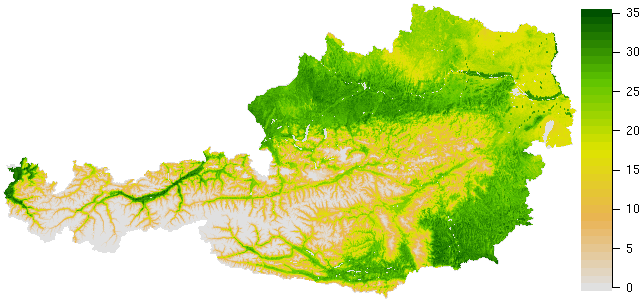
\includegraphics[width=.95\columnwidth]{./pic/quSp_t0_p1.png}
  \caption{Höhe [m] der höchsten 100 Bäume je Hektar eines Bestandes im
    Alter 100 (Oberhöhenbonität von Eiche)
    \citep[S.~17]{kindermann2021Eiche}}
  \label{fig:Eichenbonitaet}
\end{figure}

Neben diesen waldspezifischen Karten geben auch Karten zur Geologie,
Boden, Niederschlag oder Temperatur wichtige Hinweise und können oft
in Schulatlanten oder im Internet gefunden werden.


\subsection{Ökogramme}
\label{sec:oekogramme}

Ökogramme stellen auf den Achsen Bodenfeuchte (dürr--nass) und
Bodenreaktion (sauer--basisch) das Vorkommen einer Baumart dar. Dabei
wird zwischen der physiologischen Amplitude, physiologisches Optimum
und Herrschaftsbereich der Baumart, in der Regel für eine bestimmte
\emph{Höhenstufe} (Planar--subalpin), unterschieden
(Abb.\ref{fig:oekogramm}). De facto werden also 3~Dimensionen,
Feuchte, Bodenreaktion und Temperatur, dargestellt.

\begin{figure}[htbp]
  \centering
\begin{tikzpicture}
  \draw [line width=2pt] (0,0) -- (8,0) -- (8,8) -- (0,8) -- cycle;
  \draw (0,7.5) node[anchor=east] {dürr};
  \draw (0,4) node[anchor=east] {frisch};
  \draw (0,0.5) node[anchor=east] {nass};
  \draw (0.5,0) node[anchor=north,align=center] {sehr\\sauer};
  \draw (4,0) node[anchor=north,align=center] {mässig\\sauer};
  \draw (7.5,0) node[anchor=north] {basisch};
  \draw[line width=2pt,dashed] (0,7.5) -- (8,7.5);
  \draw[line width=2pt,dashed] (0,1.5) {[rounded corners=1cm] -- (1,.5)} -- (8,.5);
  %\draw[pattern=north west lines]
  \fill[gray!70] (8,2.5) {[rounded corners=1cm] -- (1.5,2.5) -- (1.5,5.5)} -- (8,5.5);
  \fill[gray!170] (8,7.3) {[rounded corners=.3cm] -- (0.3,7.3) -- (0,7)} {[rounded corners=.8cm] -- (0,4.5) -- (1.5,4.5) -- (1.5,6) -- (8,6.8)};
  \draw[line width=3pt,fill=gray,fill opacity=0.2] (8,2) -- (1,2) {[rounded corners=1cm] -- (0,2)} {[rounded corners=.3cm] -- (0,7) -- (0.3,7.3)} -- (8,7.3) -- cycle;
  \draw [line width=2pt] (4,4) circle (.1);
\end{tikzpicture}
  \caption{Beispiel eines Ökogramms}
  \footnotesize{
    \tikz \draw[line width=2pt,dashed,rounded corners=2] (0,0) rectangle (1em,1em);~Grenze waldfähiger Standorte,
    \tikz \draw[line width=3pt,fill=gray,fill opacity=0.2,rounded corners=2] (0,0) rectangle (1em,1em);~Physiologische Amplitude,
    \tikz \fill[gray!80,rounded corners=2] (0,0) rectangle (1em,1em);~Physiologisches Optimum,
    \tikz \fill[gray!160,rounded corners=2] (0,0) rectangle (1em,1em);~Herrschaftsbereich der Baumart (ökologisches Optimum / Niesche)
  }
  \label{fig:oekogramm}
\end{figure}

Ähnlich den Ökogrammen sind \emph{Klimadiagramme}, mit den Achsen
Temperatur und Niederschlag, in welche, meist als Punktwolke,
Beobachtungen einer Baumart dargestellt werden. Zwischen
pysiologischem Optimum und ökologischer Niesche wird dort meist nicht
unterschieden, da dies eben alleine über Niederschlag und Temperatur
kaum differenzierbar sein wird.

Eine Erweiterung auf zusätzliche, wesentliche Standortsdimensionen
stellen die \emph{Zeigerwerte nach Ellenberg} dar
\citep{ellenberg2010vegetation}. Mit diesen kann ein Standort,
aufgrund der auf ihm wachsenden Pflanzen, charakterisiert
werden. D.h.\ es wird in der Regel das ökologische Optimum, nicht
jedoch das physiologische Optimum oder Spektrum
dargestellt. Beschrieben werden Licht, Temperatur, Kontinentalität,
Feuchtigkeit, Bodnreaktion, Stickstoff, Salz und
Schwermetallresistenz. Weiters wird die Lebensform und die
Blattausdauer (immergrün, sommergrün, \dots) angegeben. Für Österreich
wurden diese Zeigerwerte von \cite{karrer1992Zeigerwerte} angepasst.
Ähnlich sind auch die Zeigerwerte nach
\cite{landolt2010floarIndicative} für die Schweiz oder
\cite{ehrendorfer1971NaturgechichteWiens} für Wien.

Basierend auf diesen Zeigerwerten wurde von
\cite{ninemetsValladares2006TolleranceToShadeDroughtAndWaterlogging}
nicht das häufigste Vorkommen, sonder die Grenze des Vorkommens,
hinsichtlich Trockenheit, Überschwemmung und Schatten, von mehr als
800~Baum-- und Straucharten, aufbereitet
(Tabelle:~\ref{tab:trockentolleranz}). Ein Wert von 1 bedeutet
geringe, einer von 5 hohe Toleranz.

\begin{table}[htbp!]
\centering
\begin{tabular}{l S[
  table-number-alignment = center,
  separate-uncertainty = true,
  table-figures-uncertainty = 1,
  table-figures-decimal = 2,
  table-figures-integer = 1
  ] S[
  table-number-alignment = center,
  separate-uncertainty = true,
  table-figures-uncertainty = 1,
  table-figures-decimal = 2,
  table-figures-integer = 1
  ]}
  & {Trockentoleranz} & {Schattentoleranz}\\
  \hline
  Gleditschie   & 4.98 \pm 0.02 & 1.61 \pm 0.2  \\
  Schwarzkiefer & 4.38 \pm 0.47 & 2.1  \pm 0.43 \\
  Weißkiefer    & 4.34 \pm 0.47 & 1.67 \pm 0.33 \\
  Zerreiche     & 4.29 \pm 0.21 & 2.55 \pm 0.11 \\
  Robine        & 4.11 \pm 0.65 & 1.72 \pm 0.25 \\[.3em]
  Flaumeiche    & 4.1  \pm 0.25 & 2.31 \pm 0.22 \\
  Edelkastanie  & 3.46 \pm 0.18 & 3.15 \pm 0.23 \\
  Traubeneiche  & 3.02 \pm 0.15 & 2.73 \pm 0.27 \\
  Zirbe         & 3.01 \pm 0.43 & 2.87 \pm 0.3  \\
  Nuss          & 2.98 \pm 0.22 & 2.27 \pm 0.24 \\[.3em]
  Stieleiche    & 2.95 \pm 0.31 & 2.45 \pm 0.28 \\
  Roteiche      & 2.88 \pm 0.12 & 2.75 \pm 0.18 \\
  Aspe          & 2.85 \pm 0.25 & 2.22 \pm 0.07 \\
  Winterlinde   & 2.75 \pm 0.15 & 4.18 \pm 0.16 \\
  Bergahorn     & 2.75 \pm 0.16 & 3.73 \pm 0.21 \\[.3em]
  Spitzahorn    & 2.73 \pm 0.16 & 4.2  \pm 0.37 \\
  Hainbuche     & 2.66 \pm 0.16 & 3.97 \pm 0.12 \\
  Kirsche       & 2.66 \pm 0.22 & 3.33 \pm 0.33 \\
  Douglasie     & 2.62 \pm 0.41 & 2.78 \pm 0.18 \\
  Esche         & 2.5  \pm 0.25 & 2.66 \pm 0.13 \\[.3em]
  Buche         & 2.4  \pm 0.43 & 4.56 \pm 0.11 \\
  Küstentanne   & 2.33 \pm 0.33 & 4.01 \pm 0.19 \\
  Lärche        & 2.31 \pm 0.55 & 1.46 \pm 0.29 \\
  Schwarzerle   & 2.22 \pm 0.66 & 2.71 \pm 0.5  \\
  Schwarzpappel & 2.2  \pm 0.38 & 2.46 \pm 0.09 \\[.3em]
  Hängebirke    & 1.85 \pm 0.21 & 2.03 \pm 0.09 \\
  Tanne         & 1.81 \pm 0.28 & 4.6  \pm 0.06 \\
  Fichte        & 1.75 \pm 0.41 & 4.45 \pm 0.5  \\
  Moorbirke     & 1.27 \pm 0.18 & 1.85 \pm 0.07
\end{tabular}
\caption{Trocken-- und Schattentoleranz nach \cite{ninemetsValladares2006TolleranceToShadeDroughtAndWaterlogging}.}
\label{tab:trockentolleranz}
\end{table}


\subsection{Gefährdungen}
\label{sec:gefaerdungen}

Die Dispositionierung, für bestimmte Gefahren, hängt von vielen
Faktoren ab, die oft als zufällig betrachtet werden. Es gibt immer
wieder Bestandessituationen, bei denen die Wahrscheinlichkeit, dass
ein Schaden eintritt, sehr groß ist, und dennoch wird kein Schaden
beobachtet. Umgekehrt gibt es welche, die als recht sicher gelten und
geschädigt werden. Angaben zur Gefährdung sind deshalb immer nur
\emph{Wahrscheinlichkeiten} und keine Prognosen. So zeigt etwa die
Tab.\ref{tab:gefaehrdungen}) von Wellenstein in
\citet[S.~228]{speidel1972PlanungImForstbetrieb}, Produktionsgefahren
und Risikowahrscheinlichkeiten bei verschiedenen Baumarten.

\begin{table}[htbp!]
  \setlength{\tabcolsep}{1pt}
  \centering
  \pgfplotstabletypeset[col sep=comma
  , comment chars=\#
  , text indicator="
  , string type
  , every column/.style={column type=c,preproc cell content/.style={@cell content = \rating{##1}}}
    , display columns/0/.style={column type=l,column name=\rotatebox{-90}{}, preproc cell content/.style={@cell content = ##1}}
  , assign column name/.style={/pgfplots/table/column name={\multicolumn{1}{c}{\rotatebox{90}{#1}}}}
  ]{./tabs/gefaehrdung.csv}
  \caption{Produktionsgefahren und Risikowahrscheinlichkeiten bei verschiedenen
    Baumarten nach Wellenstein in \cite{speidel1972PlanungImForstbetrieb}}
  \footnotesize{\rating{0}\dots keine Gefährdung,
    \rating{1}\dots wirtschaftl.\ unbedeutende Gefährdung,
    \rating{2}\dots w.\ bedeutende Gefährdung,
    \rating{3}\dots w.\ sehr bedeutende Gefährdung}
  \label{tab:gefaehrdungen}
\end{table}



%https://klimadatenportal.lgl-bw.de/viewer/client/index.html


%\addcontentsline{toc}{section}{Stichwortverzeichnis}
%\printindex

\addcontentsline{toc}{section}{Literatur}
\bibliography{literature}

\clearpage % To flush out all floats

\begin{table*}[htbp!]
  \setlength{\tabcolsep}{1pt}
  %\centering
  \pgfplotstabletypeset[col sep=comma
  , text indicator="
  , string type
  , every column/.style={column type=c,preproc cell content/.style={@cell content = \ratingB{##1}{2}}}
  , my colIterator/.style={every col no #1/.style={column type=c,preproc cell content/.style={@cell content = \ratingB{####1}{3}}}}
  , my colIterator/.list={1,2,11,16}
  , my colIteratorB/.style={every col no #1/.style={column type=c,preproc cell content/.style={@cell content = \ratingB{####1}{4}}}}
  , my colIteratorB/.list={10,15}
  , display columns/5/.style={column type=c|,preproc cell content/.style={@cell content = \ratingB{##1}{4}}}
  , display columns/9/.style={column type=c||,preproc cell content/.style={@cell content = \ratingB{##1}{3}}}
  , display columns/19/.style={column type=c,preproc cell content/.style={@cell content = \ratingB{\the\numexpr ##1 - 410 \relax}{340}}}
  , display columns/0/.style={column type=l,column name=\rotatebox{-90}{}, preproc cell content/.style={@cell content = ##1}}
  , assign column name/.style={/pgfplots/table/column name={ \multicolumn{1}{c}{\rotatebox{90}{#1}}}}
  , every row no 0/.append style={before row={
      & \multicolumn{5}{c|}{Anspruch} & \multicolumn{4}{c||}{Empfindl.}
      & \multicolumn{9}{c}{Eigenschaft} \\
     }}
  ]{./tabs/baCharakter.csv}
  \caption{Ansprüche und Eigenschaften heimischer Wirtschaftsbaumarten nach \citet[Bd.1, S.183f]{bauer1962WaldbauAlsWissenschaft}}
  \footnotesize{\emph{Anspruch, Empfindlichkeit, Eigenschaft:} \ratingB{0}{3}\dots gering, \ratingB{1}{3}\dots mäßig, \ratingB{2}{3}\dots hoch, \ratingB{3}{3}\dots sehr hoch\\
    \emph{Verhalten zu Nachbarn:} \ratingB{0}{2}\dots unverträglich, \ratingB{1}{2}\dots störend, \ratingB{2}{2}\dots verträglich
  }  
  \label{tab:baCharakter}
\end{table*}

\afterpage{%
%  \clearpage% To flush out all floats
\begin{landscape}
  \begin{figure}[h]
    \centering
    \includegraphics[height=.9\textheight]{./pic/waelderDesOstalpenraumes.pdf}
    \caption{Wälder des Ostalpenraumes \citep{mayer1977KarteWaldtypen}}
    \label{fig:waelderDesOstalpenraumes}
  \end{figure}
\end{landscape}
}

\begin{table*}[htbp!]
  \setlength{\tabcolsep}{1pt}
  \centering
  \pgfplotstabletypeset[col sep=comma
  , text indicator="
  , string type
  , after row=\cdashline{3-38}
  %, every head row/.style={before row=\hline}
  %, every last row/.style={after row={}}
  %, every last column/.style={column type=c}
  , every column/.style={column type=c:,preproc cell content/.style={@cell content = \torte{##1}}}
  , display columns/0/.style={column type=l,column name=\rotatebox{-90}{Waldgesellschaft}, preproc cell content/.style={@cell content = ##1}}
  , display columns/1/.style={column type=c|,preproc cell content/.style={@cell content = \hst{##1}}}
  , assign column name/.style={/pgfplots/table/column name={\multicolumn{1}{c}{\rotatebox{90}{#1}}}}
  , columns/Weisskiefer/.style={column name=Weißkiefer}
  , every row no 4/.style={before row=\hline}
  , every row no 12/.style={before row=\hline}
  , every row no 22/.style={before row=\hline}
  ]{./tabs/gesselschaftsanschluss.csv}
  \caption{Natürlicher Gesellschaftsanschluß mit Vergesellschaftung der Baumarten in Wäldern des Ostalpenraumes \citep{mayer1992Waldbau}}
  \footnotesize{\hst{0}\dots Auwald,
    \hst{1}\dots Planar--Kolin --400\,m,
    \hst{2}\dots Submontan 200--900\,m,
    \hst{3}\dots Montan 500--1800\,m,
    \hst{4}\dots Subalpin 1200--2300\,m\\
    \tikz \draw (0,0) rectangle (1em,1em);\dots fehlend,
    \torte{1}\dots sporadisch,
    \torte{2}\dots spärlich,
    \torte{3}\dots gering,
    \torte{4}\dots mittel,
    \torte{5}\dots reichlich,
    \torte{6}\dots vorherschend
  }
  \label{tab:waldgesellschaften}
\end{table*}

%\begin{table*}[htbp!]
%  \setlength{\tabcolsep}{1pt}
%  %\centering
%  \pgfplotstabletypeset[col sep=comma
%  , text indicator="
%  , string type
%  ]{./tabs/baEigenschaften.csv}
%  \caption{Eigenschaften}
%  \footnotesize{\emph{Eigenschaft:} \ratingB{0}{3}\dots gering, \ratingB{1}{3}\dots mäßig, \ratingB{2}{3}\dots hoch, \ratingB{3}{3}\dots sehr hoch\\
%  }  
%  \label{tab:baEigenschaften}
%\end{table*}

%\begin{table*}[htbp!]
%  \setlength{\tabcolsep}{1pt}
%  %\centering
%  \pgfplotstabletypeset[col sep=comma
%  , text indicator="
%  , string type
%  ]{./tabs/baAnspruch.csv}
%  \caption{Ansprüche}
%  \footnotesize{\emph{Anspruch:} \ratingB{0}{3}\dots gering, \ratingB{1}{3}\dots mäßig, \ratingB{2}{3}\dots hoch, \ratingB{3}{3}\dots sehr hoch\\
%  }  
%  \label{tab:baAnsprueche}
%\end{table*}

%\begin{table*}[htbp!]
%  \setlength{\tabcolsep}{1pt}
%  %\centering
%  \pgfplotstabletypeset[col sep=comma
%  , text indicator="
%  , string type
%  ]{./tabs/baEmpfindlichkeiten.csv}
%  \caption{Empfindlichkeiten}
%  \footnotesize{\emph{Empfindlichkeit:} \ratingB{0}{3}\dots gering, \ratingB{1}{3}\dots mäßig, \ratingB{2}{3}\dots hoch, \ratingB{3}{3}\dots sehr hoch\\
%  }  
%  \label{tab:baEmpfindlichkeiten}
%\end{table*}

\newpage

% \includepdf[pages=-,pagecommand={},width=\textwidth]{test.pdf}

\tablecaption{Charakteristika einiger Baumarten}
\label{tab:BaumartenCharakteristik}
\tablehead{Code & Art Sci & Kurz & Art & t & H & h & A & X & D & T & K & W & L & R & N & F & Ü & G & Z & U & a & w & d & x & M & V & F & S & I & B & P\\ \hline \noalign{\vskip .1em}}
\tabletail{\hline Code & Art Sci & Kurz & Art & t & H & h & A & X & D & T & K & W & L & R & N & F & Ü & G & Z & U & a & w & d & x & M & V & F & S & I & B & P\\}
\tablelasttail{Code & Art Sci & Kurz & Art & t & H & h & A & X & D & T & K & W & L & R & N & F & Ü & G & Z & U & a & w & d & x & M & V & F & S & I & B & P\\}

\afterpage{%
  \onecolumn
  \begin{landscape}
    \begin{xtabular}{llllcccccc@{$\cdot$}cccccc@{$\cdot$}ccc@{$\cdot$}cccccc@{$\cdot$}cccc@{$\cdot$}ccc}
      \input{./rtab/SpTab.tex}\\
      \hline
    \end{xtabular}\\
    \footnotesize{
      Code\dots Baumartencode in Anlehnung an EN~13556\\
      Art Sci\dots Wissenschaftlicher Name\\
      Kurz\dots Baumartencode in Anlehnung an DIN~4076\\
      Art\dots Deutscher Name\\
      t\dots Typ: \typ{1}{0}\dots Nadel sommergrün,
      \typ{1}{1}\dots Nadel immergrün,
      \typ{2}{0}\dots Laub sommergrün,
      \typ{2}{1}\dots Laub immergrün,
      \typ{3}{0}\dots Gingko
      \typ{4}{0}\dots Kletterpflanze sommergrün,
      \typ{4}{1}\dots Kletterpflanze immergrün,
      \typ{5}{0}\dots Palme,
      \typ{6}{0}\dots Kaktus\\
      H\dots Höhe die auf guten Standorten erreicht werden kann: \ratingC{0}{25}\dots 15\,m, \ratingC{0}{50}\dots 30\,m, \ratingC{0}{75}\dots 45\,m, \ratingC{0}{100}\dots 60\,m oder mehr\\
      h\dots Höhe die im Alter~15 auf guten Standorten erreicht werden kann: \ratingC{0}{25}\dots 4\,m, \ratingC{0}{50}\dots 8\,m, \ratingC{0}{75}\dots 12\,m, \ratingC{0}{100}\dots 16\,m oder mehr\\
      A\dots Erreichbares Alter: \ratingC{0}{25}\dots 100~Jahre, \ratingC{0}{50}\dots 200~Jahre, \ratingC{0}{75}\dots 300~Jahre, \ratingC{0}{100}\dots 400~Jahre oder mehr\\
      X\dots Niesche: \ratingC{0}{0}\dots Pionier, \ratingC{0}{50}\dots Extramstandort, \ratingC{0}{100}\dots Konkurrenzstark\\
      D\dots Durchwurzelungstiefe: \ratingC{0}{33}\dots 1\,m, \ratingC{0}{67}\dots 2\,m, \ratingC{0}{100}\dots 3\,m oder mehr\\
      T\dots Temperatur: \ratingC{0}{0}\dots Sehr Kälteempfindlich, \ratingC{0}{100}\dots Geringe Kälteempfindlichkeit\\
      K\dots Kontinentalität: \ratingC{0}{0}\dots Verträgt nur geringe Temperaturschwankung (ozeanisch), \ratingC{0}{100}\dots Verträgt größe Temperaturschwankungen (kontinental)\\
      W\dots Wasser: \ratingC{0}{20}\dots Verträgt Stauwasser, \ratingC{40}{60}\dots frisch (nicht trocken und nicht nass), \ratingC{80}{100}\dots Verträgt Trockenheit\\
      L\dots Licht:  \ratingC{0}{0}\dots Benötigt viel Licht, \ratingC{0}{100}\dots Erträgt starke Beschattung\\
      R\dots Bodenreaktion: \ratingC{0}{10}\dots Stark saure Böden (silikat), \ratingC{40}{60}\dots neutrale Böden, \ratingC{80}{100}\dots Sehr basische Böden (kalk)\\
      N\dots Nährstoffbedarf: \ratingC{0}{0}\dots Sehr hoch, \ratingC{0}{100}\dots Sehr Gering\\
      F\dots \jaNeinQ{0}{0}{0}{1}\dots Stickstofffixierung,
      \jaNeinQ{0}{0}{1}{0}\dots Windbestäubt,
      \jaNeinQ{1}{0}{0}{0}\dots Salzresistent,
      \jaNeinQ{0}{1}{0}{0}\dots Schwermetallresistent\\
      Ü\dots Überdauerungszeitraum von Samen: \ratingC{0}{25}\dots 25~Jahre, \ratingC{0}{50}\dots 50~Jahre, \ratingC{0}{75}\dots 75~Jahre, \ratingC{0}{100}\dots 100~Jahre oder mehr\\
      G\dots Als Nahrung verwendet / Giftig : \jaNeinP{0}{1}\dots Als Nahrung verwendet. Dies bedeuted \textbf{nicht}, das diese Pflanze ohne Gefahr essbar ist.
      \jaNeinP{1}{0}\dots Giftig. Ungiftig wurde hier nicht vergeben! D.h.\ keine Angabe bedeuted \textbf{nicht}, das diese Pflanze ohne Gefahr essbar ist.\\
      Z\dots Planbarkeit: \ratingC{0}{10}\dots Gering --
      Wahrscheinlichkeit für frühzeitigen Ausfall, \ratingC{0}{90}\dots Hoch\\
      U\dots Streuumsatz: \ratingC{0}{0}\dots 5~Jahre oder mehr, \ratingC{0}{100}\dots 1~Jahr oder weniger\\
      a\dots Stockausschlag: \ratingC{0}{0}\dots Nein, \ratingC{0}{100}\dots Ja\\
      w\dots Wurzelbrut: \ratingC{0}{0}\dots Nein, \ratingC{0}{100}\dots Ja\\
      d\dots Holzichte: \ratingC{0}{0}\dots Darrgewicht 350 kg/m$^3$ oder weniger, \ratingC{0}{100}\dots Darrgewicht 800 kg/m$^3$ oder mehr\\
      x\dots Dauerhaftigkeit des unbehandelten Kern--Holzes in Anlehnung an EN 350-2: \ratingC{0}{0}\dots geringe Dauerhaftigkeit, \ratingC{0}{100}\dots Sehr Dauerhaft\\
      M\dots Mäuse: \ratingC{0}{0}\dots geringe Gefährdung, \ratingC{0}{100}\dots hohe Gefährdung\\
      V\dots Verbiss: \ratingC{0}{0}\dots geringe Gefährdung, \ratingC{0}{100}\dots hohe Gefährdung\\
      F\dots Fegen/Schlagen: \ratingC{0}{0}\dots geringe Gefährdung, \ratingC{0}{100}\dots hohe Gefährdung\\
      S\dots Schälen: \ratingC{0}{0}\dots geringe Gefährdung, \ratingC{0}{100}\dots hohe Gefährdung\\
      I\dots Windwurf: \ratingC{0}{0}\dots geringe Gefährdung, \ratingC{0}{100}\dots hohe Gefährdung\\
      B\dots Schneebruch: \ratingC{0}{0}\dots geringe Gefährdung, \ratingC{0}{100}\dots hohe Gefährdung\\
      P\dots Pilze: \ratingC{0}{0}\dots geringe Gefährdung, \ratingC{0}{100}\dots hohe Gefährdung\\
    }
  \end{landscape}
  \twocolumn
}

  
%Autor: Georg Kindermann

\end{document}
